\section{Exploración}
Los datos proporcionados vienen en dos tablas separadas:

\begin{itemize}
    \item La tabla \textit{identity}, que recoge información sobre
    los usuarios que realizan las transacciones (tipo de dispositivo,
    dirección, \dots).
    \item La tabla \textit{transaction}, que es la que tiene las
    transacciones como tales (tiempo, cantidad de dinero, producto
    comprado, tarjeta usada, \dots), además de la clase objetivo
    \textit{isFraud}.
\end{itemize}

Ambas tablas tienen en común un atributo \textit{TransactionID}, que usamos para
unirlas. Hay que tener en cuenta que no todas las transacciones de la tabla
\textit{transaction} tienen una identidad asociada, por lo que la unión que
realizamos es de tipo \textit{innerjoin}, quedándonos solo con los registros de
transacciones que tienen identidad.

\begin{lstlisting}
library(tidyverse)

if (!file.exists("data/train_innerjoin.csv") || !file.exists("data/test_innerjoin.csv")) {
  # Load train and test source datasets
  train_transaction <- read_csv("data/train_transaction.csv")
  train_identity <- read_csv("data/train_identity.csv")
  test_transaction <- read_csv("data/test_transaction.csv")
  test_identity <- read_csv("data/test_identity.csv")
  
  # Merge tables
  train_dataset <- merge(train_transaction, train_identity, by = "TransactionID")
  test_dataset <- merge(test_transaction, test_identity, by = "TransactionID")
  
  # Write merged datasets
  write_csv(train_dataset, "data/train_innerjoin.csv")
  write_csv(test_dataset, "data/test_innerjoin.csv")
} else {
  # Load train and test datasets
  train_dataset <- read_csv("data/train_innerjoin.csv")
  test_dataset <- read_csv("data/test_innerjoin.csv")
}
\end{lstlisting}

Como se puede apreciar en el código encargado de leer los datos y unir las
tablas, tenemos datos tanto de \textit{train} como de \textit{test}. No
obstante, los datos de \textit{test} no contienen la clase objetivo, ya que
están pensados para usarse en la competición de kaggle enviando los resultados
obtenidos de las predicciones realizadas sobre este conjunto y obteniendo las
métricas de calidad de la predicción. Como la competición ya ha finalizado, este
conjunto no nos es realmente útil, por lo que a partir de ahora trabajaremos
solo sobre el de \textit{train}.

En este conjunto de datos tenemos un total de 434 variables y 144233 registros
tras la unión de las tablas. Son muchísimos datos, por lo que tendremos que
realizar una extracción de variables para reducir su número. Si no hiciéramos
esto, los tiempos de ejecución y requisitos de memoria serían demasiado altos.
Entre estas variables tenemos la clase objetivo \textit{isFraud}, dos variables
continuas (\textit{TransactionDT} y \textit{TransactionAmt}) que tendremos que
convertir a intervalos y una serie de variables que sabemos que son categóricas
gracias a que así lo indica la competición en kaggle, ya que observando los
datos podrían parecer numéricas. Cabe destacar que, debido al carácter sensible
de los datos, el significado de muchas de las variables está enmascarado y, por
lo tanto, no podemos conocerlo.

Para conocer más información sobre los datos, usamos la función
\lstinline{df_status()} del paquete \textit{funModeling}, con la que podemos ver
el porcentaje de valores NA y la dispersión de las variables del conjunto de
datos. En la figura \ref{fig:na-barplot}, podemos ver que hay una gran cantidad
de NAs, habiendo variables con más de un 50\% de estos valores. Todas estas
variables que tienen muchos valores vacíos podremos eliminarlas en favor de otras
que tienen más información. También podemos ver, en la figura
\ref{fig:dispersity-barplot}, el porcentaje de dispersión de los valores de las
distintas variables. Se puede apreciar como hay una variable con una dispersión
extremadamente alta, que llega hasta el 80\%. Si quitamos esta variable, en la
figura \ref{fig:dispersity-reduced-barplot} vemos que también tenemos variables
con una dispersión muy baja, incluso llegando al 0\%. Todas estas variables de
dispersión elevada o muy baja las podremos eliminar del conjunto de datos.

\begin{figure}
    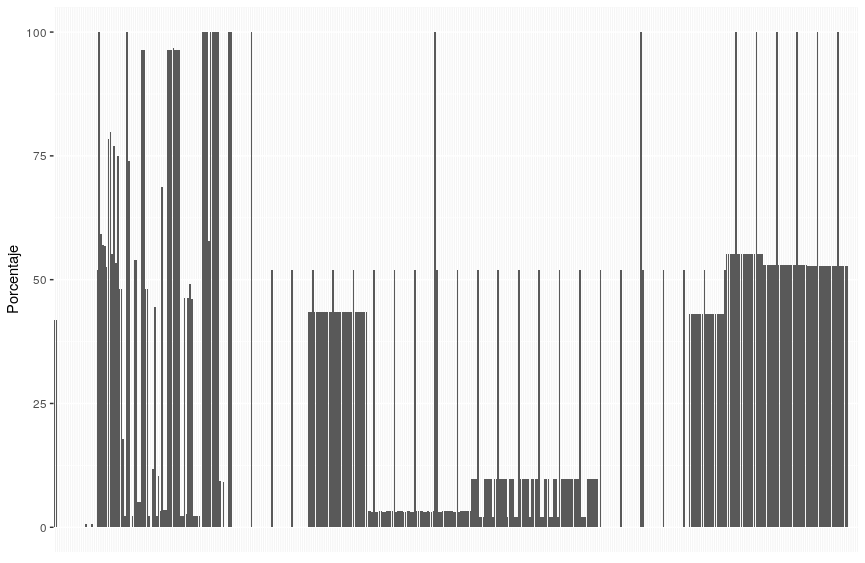
\includegraphics[width=\textwidth]{images/exploration/na-barplot.png}
    \caption{Porcentaje de valores NA por variable.}
    \label{fig:na-barplot}
\end{figure}

\begin{figure}
    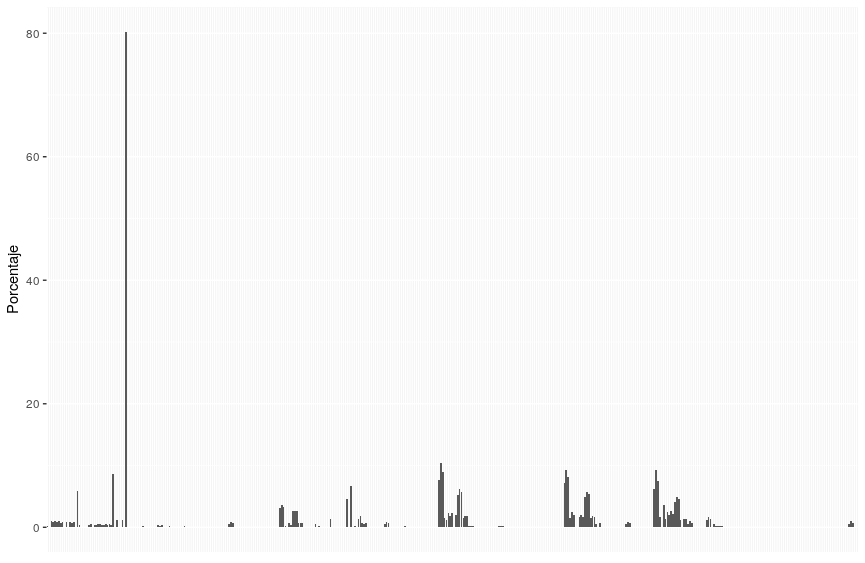
\includegraphics[width=\textwidth]{images/exploration/dispersity-barplot.png}
    \caption{Porcentaje de dispersión de valores.}
    \label{fig:dispersity-barplot}
\end{figure}

\begin{figure}
    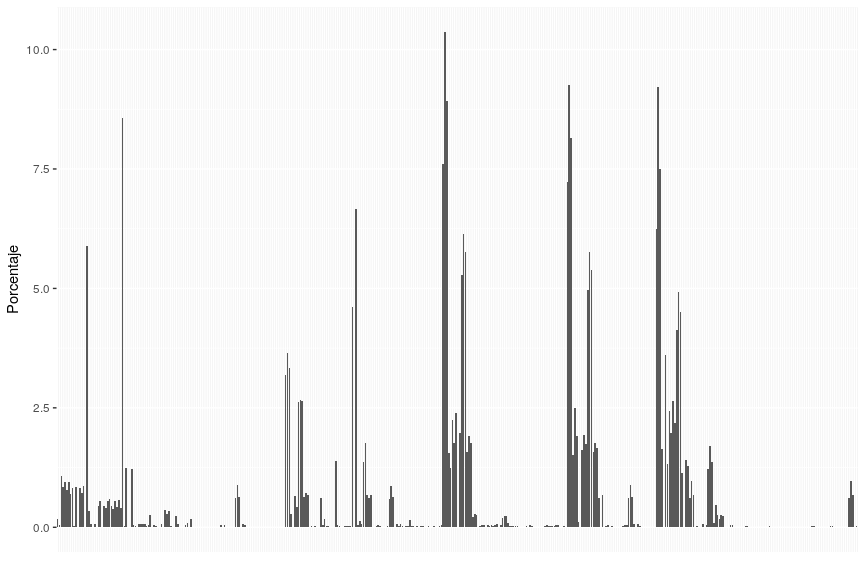
\includegraphics[width=\textwidth]{images/exploration/dispersity-reduced-barplot.png}
    \caption{Porcentaje de dispersión de valores para variables con dispersión inferior al 60\%.}
    \label{fig:dispersity-reduced-barplot}
\end{figure}

También podemos fijarnos en la correlación entre variables para ver si hay
algunas que podamos eliminar. Si dos variables están muy correladas, podremos
eliminar una de ellas, ya que ambas nos aportarían la misma información. En la
figura \ref{fig:correlation-heatmap} tenemos un mapa de calor que refleja las
correlaciones entre las variables de tipo numérico del conjunto de datos. Las
zonas con un tono más claro indican una alta correlación, por lo que serían
pares de variables a considerar.

\begin{figure}
    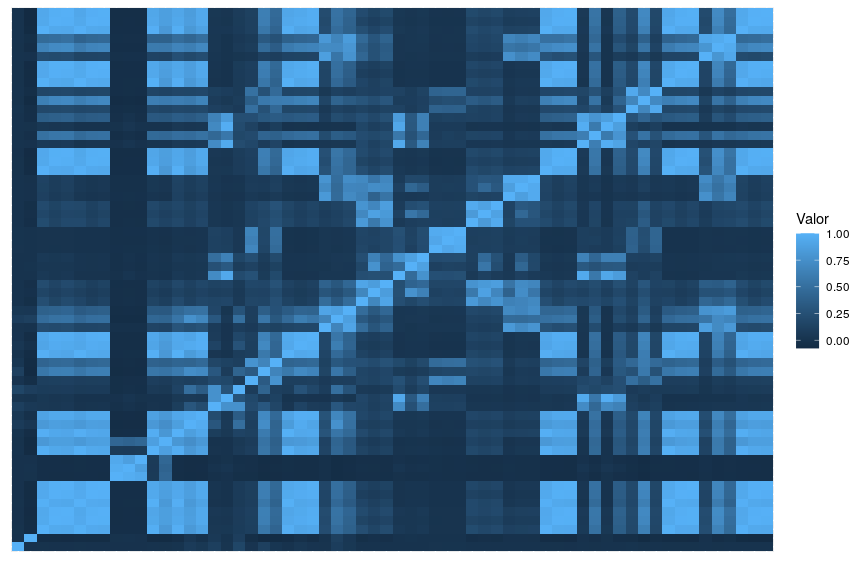
\includegraphics[width=\textwidth]{images/exploration/correlation-heatmap.png}
    \caption{Correlación entre variables numéricas.}
    \label{fig:correlation-heatmap}
\end{figure}

Para terminar con la exploración, podemos observar el número de registros
que tenemos para cada valor de la clase objetivo \textit{isFraud}, lo cuál
podemos ver en la figura \ref{fig:class-barplot}. Como era de esperar, hay
muchos más ejemplos de transacciones que no son fraude que de las que sí lo son,
ya que estas últimas son menos frecuentes. Para entrenar los clasificadores,
necesitaremos balancear el conjunto de datos primero.

\begin{figure}
    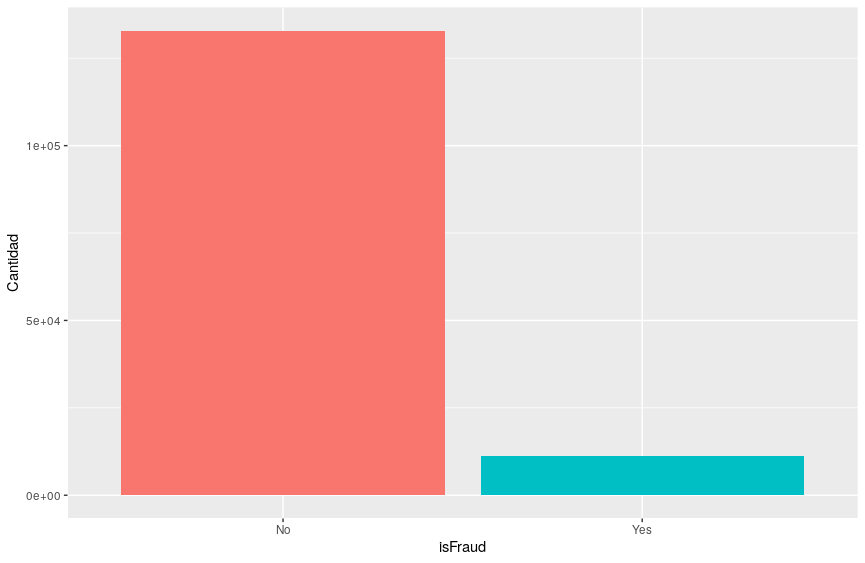
\includegraphics[width=\textwidth]{images/exploration/class-barplot.png}
    \caption{Cantidad de ejemplos de cada valor de la clase objetivo presentes en el conjunto de datos.}
    \label{fig:class-barplot}
\end{figure}
